% Provenance (never printed): cycle 3 "Matiere, mouvement, energie,
% information" and "La planete Terre" (meteorological phenomena, the water in
% the air, measuring the weather); see sources/book1/PROVENANCE.md.
% Book 1, grade 4, chapter 1.
\chapter{云、雨和雪}\label{ch:g4:clouds-rain-snow}

这是一个炎热的夏日午后。午饭时，天空湛蓝，
飘着几朵小小的白云，像一团团棉花球。
到三点钟时，其中一朵长大了，不断向上膨胀，越升越高，像一株白色花椰菜。
它立在扁平的灰色底座上。云顶向四周铺展开来，云底变成了暗色。
一阵凉风吹过，第一批大雨滴落下，接着整整下了二十分钟。
然后云飘走了，太阳重新露面，
湿漉漉的人行道冒起了水蒸气。

那朵云从哪里来？它由什么构成？
这二十分钟里一共下了多少雨？

\begin{recall}
\omterm{def:g1:watching-the-weather:weather}{天气}是指某一地点、某一时刻的空气状态：晴朗、多云、下雨、下雪、刮风、有雾，
人们把它记录在\omterm{def:g1:watching-the-weather:weather-chart}{天气图}上，
（见\cref{ch:g1:watching-the-weather}）。\omterm{def:g2:water-on-earth:ocean}{海洋}、\omterm{def:g1:landscapes-around-us:water}{湖泊}和地面的水会蒸发进入空气，
再以雨的形式落回地面（见\cref{ch:g2:water-on-earth}）。
物理书中讲了水如何蒸发（由液体变为看不见的气体）、
如何凝结（由气体变为细小水滴）、
如何凝固（由液体变为冰），以及温度计如何测量温度，
单位为摄氏度。
\end{recall}

\section{什么是云？}

我们周围的空气中总含有一些水，它以看不见的气体形式存在，即水蒸气。
空气上升时会变冷。当温度降得足够低时，
一部分水蒸气会凝结成非常微小的水滴，
微小到连轻微的气流都能使其漂浮在空中。
无数这样的水滴聚集在一起，形成了我们能看见的云。
在高空，气温极低，水滴会凝固，云由细小的冰粒构成。

\begin{definition}[云与雾]\label{def:g4:clouds-rain-snow:cloud}
\emph{云}\index{云}是大量在空中漂浮的微小水滴，
或微小冰粒的集合，\emph{雾}\index{雾}是
接触地面的云。
\end{definition}

\begin{example}[清晨的呼吸]\label{ex:g4:clouds-rain-snow:breath}
寒冷的早晨，你呼出的气息会在嘴前形成一小团白色的云。
呼出的空气温暖，含有水蒸气。
冷空气立刻使其降温，水蒸气凝结成细小水滴——
一朵微型云出现了，随后水滴又蒸发，云便消失了。
\end{example}

云呈白色，是因为其中的水滴把阳光向四面八方散射。
云很厚时，只有很少的光能到达云底，
从下方看，云呈灰色，甚至接近黑色，
这正是满含水分的厚重\omterm{def:g4:clouds-rain-snow:cloud}{云层}的标志。

\section{云的家族}

云的形态多种多样，世界各地的气象观测员都用同样的方法为它们分类，
依据是云的形状以及它们漂浮的高度。

\begin{definition}[云族]\label{def:g4:clouds-rain-snow:cloud-families}
需要掌握的四个云族是：
\begin{itemize}
  \item \emph{积云}\index{积云}：堆积状的白色蓬松云，
        底部平坦，像一团团棉花球；
  \item \emph{层云}\index{层云}：层状云，是一片平坦的灰色云幕，
        覆盖整个天空，位置较低；
  \item \emph{卷云}\index{卷云}：丝缕状的云，像细细的白色丝线或卷曲的线条，
        位置很高，由冰构成；
  \item \emph{积雨云}\index{积雨云}：风暴云，是一座巨大的云塔，
        从低处的暗色云底一直升到很高的地方，
        其顶部常常向四周铺展成平顶。
\end{itemize}
\end{definition}

这些名称都是拉丁词：\emph{cumulus} 意为“堆”，\emph{stratus} 意为
“层”，\emph{cirrus} 意为“卷发”，\emph{nimbus} 意为“雨云”。

\begin{omfigure}
\begin{minipage}[b]{0.49\linewidth}\centering
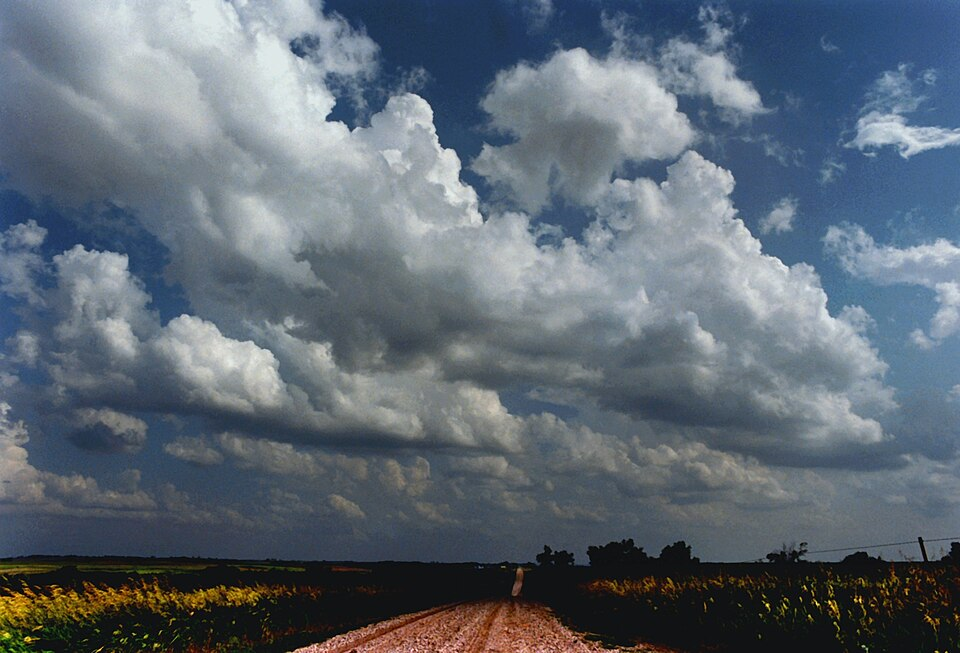
\includegraphics[width=\linewidth]{images/book1/g4-cumulus.jpg}

{\small \omterm{def:g4:clouds-rain-snow:cloud-families}{积云}：堆状云，底部平坦。}
\end{minipage}\hfill
\begin{minipage}[b]{0.49\linewidth}\centering
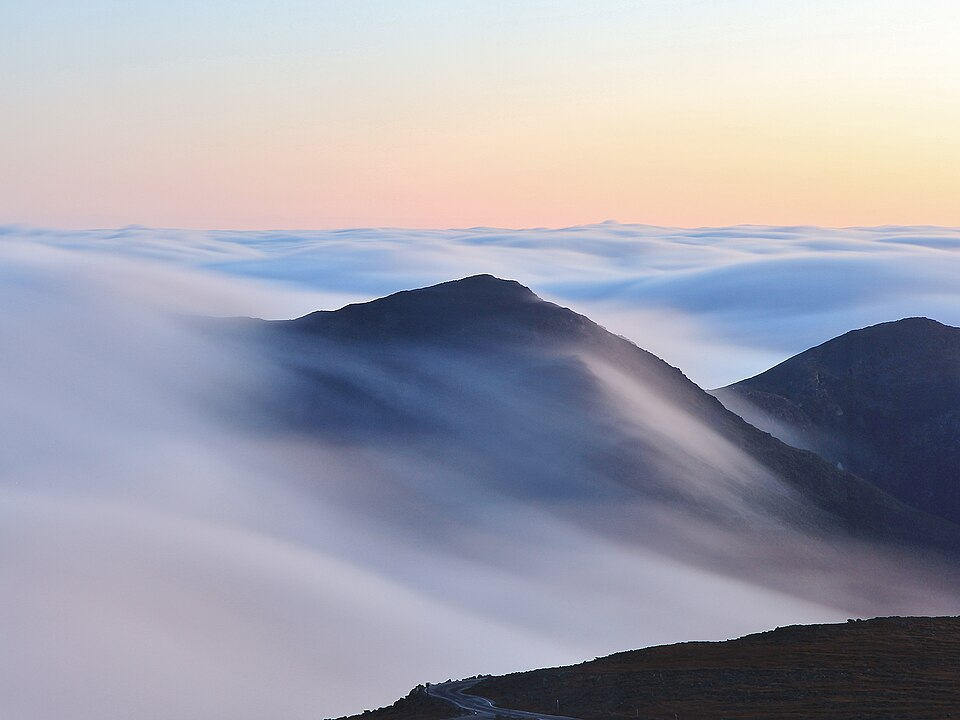
\includegraphics[width=\linewidth]{images/book1/g4-stratus.jpg}

{\small \omterm{def:g4:clouds-rain-snow:cloud-families}{层云}：平坦的\omterm{def:g4:clouds-rain-snow:cloud}{云层}，图中为从山上俯视所见。}
\end{minipage}

\medskip
\begin{minipage}[b]{0.49\linewidth}\centering
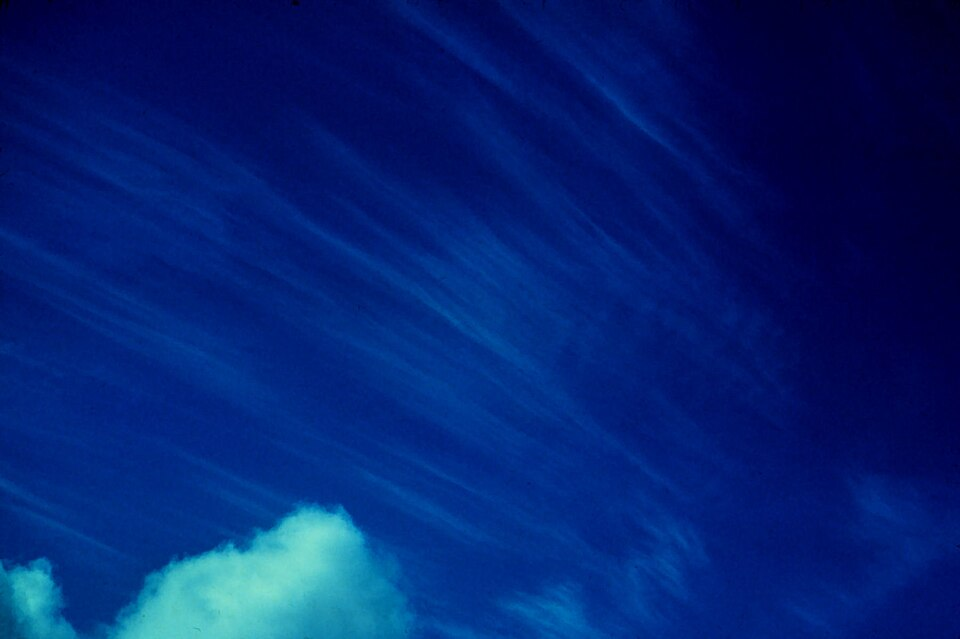
\includegraphics[width=\linewidth]{images/book1/g4-cirrus.jpg}

{\small \omterm{def:g4:clouds-rain-snow:cloud-families}{卷云}：很高处的细小冰丝（下方是一朵小\omterm{def:g4:clouds-rain-snow:cloud-families}{积云}）。}
\end{minipage}\hfill
\begin{minipage}[b]{0.49\linewidth}\centering
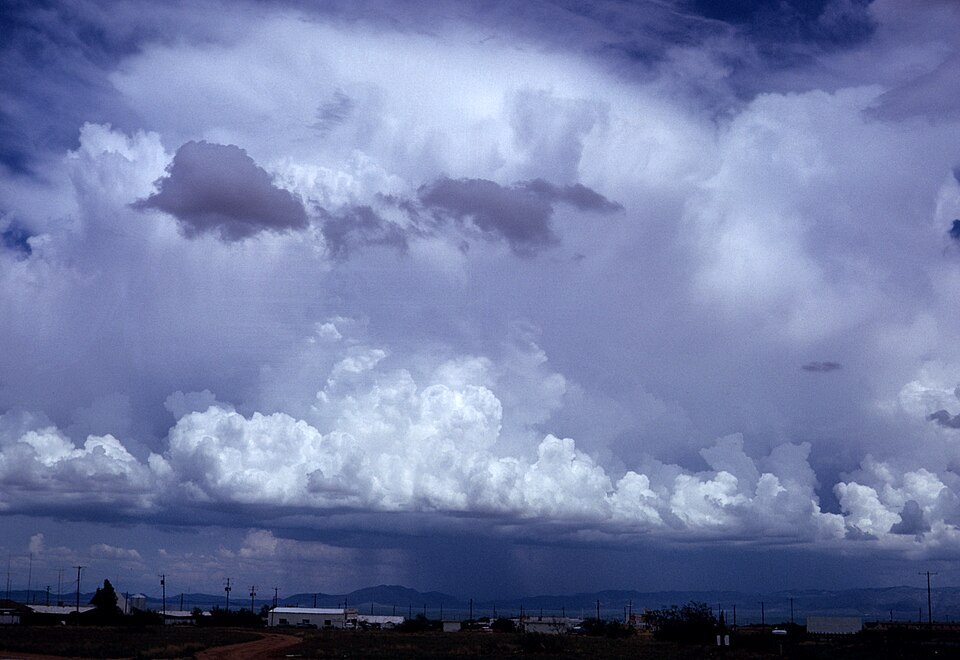
\includegraphics[width=\linewidth]{images/book1/g4-cumulonimbus.jpg}

{\small \omterm{def:g4:clouds-rain-snow:cloud-families}{积雨云}：云塔，雨从其暗色的云底落下。}
\end{minipage}

\smallskip
{\small 照片：NOAA Photo Library（公有领域）：S. Corfidi
（\omterm{def:g4:clouds-rain-snow:cloud-families}{积云}）、R. F. Kresge（\omterm{def:g4:clouds-rain-snow:cloud-families}{卷云}）、B. 胡克 collection（\omterm{def:g4:clouds-rain-snow:cloud-families}{积雨云}）。}
% ledger: noaa:photos-g4
\label{fig:g4:clouds-rain-snow:photos}
\end{omfigure}

云能漂浮到多高？这取决于云的种类。
低云，如\omterm{def:g4:clouds-rain-snow:cloud-families}{层云}和\omterm{def:g4:clouds-rain-snow:cloud-families}{积云}的云底，漂浮在贴近地面之处至
约 2 千米的高度；\omterm{def:g4:clouds-rain-snow:cloud-families}{卷云}漂浮得很高，约在 5 至 13
千米的高空（在回归线和极地地区以外）——
常常比地球上最高的山还要高。
\omterm{def:g4:clouds-rain-snow:cloud-families}{积雨云}从低处的云底一直延伸到
\omterm{def:g4:clouds-rain-snow:cloud}{云层}的最高处。
% ledger: wmo:cloud-levels, wmo:cumulonimbus

\begin{omfigure}
\begin{tikzpicture}[x=1cm, y=0.5cm, font=\small]
  % height scale
  \draw[black!60] (0,0) -- (0,14);
  \foreach \h in {0,2,...,14} {
    \draw[black!60] (-0.1,\h) -- (0,\h);
    \node[anchor=east, font=\scriptsize] at (-0.12,\h) {\h\,千米};
  }
  \node[anchor=south, font=\scriptsize, align=center] at (0,14.2) {高度};
  % ground and a mountain for comparison
  \fill[green!35!black!50] (0.2,0) -- (11.4,0) -- (11.4,-0.4) -- (0.2,-0.4) -- cycle;
  \fill[black!35] (8.6,0) -- (9.9,8.8) -- (10.2,8.4) -- (11.2,0) -- cycle;
  \fill[white, draw=black!45, line width=0.3pt] (9.65,7.2) -- (9.9,8.8) -- (10.2,8.4) -- (10.4,7.0) -- (10.1,7.4) -- (9.9,7.0) -- cycle;
  \node[font=\scriptsize, align=center] at (9.9,10.2) {最高 \\山};
  % levels
  \fill[blue!6] (0.2,0.15) rectangle (8.3,2);
  \fill[blue!10] (0.2,5) rectangle (8.3,13);
  \node[anchor=west, font=\scriptsize, text=blue!50!black] at (0.3,1.65) {低云};
  \node[anchor=west, font=\scriptsize, text=blue!50!black] at (0.3,12.6) {高云};
  % stratus: a flat grey layer
  \fill[black!25, rounded corners=2pt] (0.6,0.6) rectangle (2.6,1.3);
  \node[font=\scriptsize] at (1.6,-1.1) {层云};
  % cumulus
  \pic[scale=0.7, transform shape] at (4.0,0.9) {puffycloud};
  \node[font=\scriptsize] at (4.0,-1.1) {积云};
  % cirrus: wisps
  \foreach \y in {9.4,10.0,10.6} {
    \draw[black!50, line width=0.6pt] (0.8,\y) .. controls (1.4,\y+0.5) and (2.0,\y+0.1) .. (2.6,\y+0.6);
  }
  \node[font=\scriptsize] at (1.7,8.5) {卷云};
  % cumulonimbus: tower with an anvil
  \fill[black!15, draw=black!45, line width=0.4pt]
    (5.4,1.0) .. controls (5.2,4) and (5.6,8) .. (5.9,11.2)
    .. controls (5.0,11.6) and (4.6,12.0) .. (4.8,12.3)
    -- (8.1,12.3) .. controls (8.2,12.0) and (7.8,11.6) .. (7.0,11.2)
    .. controls (7.3,8) and (7.6,4) .. (7.4,1.0) -- cycle;
  \fill[black!45] (5.4,1.0) rectangle (7.4,1.4);
  \foreach \x in {5.7,6.1,6.5,6.9,7.2}
    \draw[omWxRain, line width=0.6pt] (\x,0.95) -- (\x-0.15,0.15);
  \node[font=\scriptsize] at (6.4,-1.1) {积雨云};
\end{tikzpicture}

{\small 四类云的漂浮高度（单位为千米，适用于
既非热带也非极地的地区）。\omterm{def:g4:clouds-rain-snow:cloud-families}{层云}和\omterm{def:g4:clouds-rain-snow:cloud-families}{积云}的云底
位置较低；\omterm{def:g4:clouds-rain-snow:cloud-families}{卷云}常常比最高的山还要高。
\omterm{def:g4:clouds-rain-snow:cloud-families}{积雨云}从低处的云底延伸到\omterm{def:g4:clouds-rain-snow:cloud}{云层}的最高处。
高度依据世界气象组织的云图谱。}
\label{fig:g4:clouds-rain-snow:heights}
% ledger: wmo:cloud-levels, tht:everest
\end{omfigure}

\begin{method}[识别云]\label{met:g4:clouds-rain-snow:naming}
观察天空，并问自己三个问题：
\begin{enumerate}
  \item 它是否是底部平坦的一堆？如果是，则为\omterm{def:g4:clouds-rain-snow:cloud-families}{积云}——若它
        升成巨大的深色塔状，则为\omterm{def:g4:clouds-rain-snow:cloud-families}{积雨云}。
  \item 它是否是平坦、均匀、遮住全天空的一层？如果是，则为
        \omterm{def:g4:clouds-rain-snow:cloud-families}{层云}。
  \item 它是否是高空中由细白丝缕构成的？如果是，则为\omterm{def:g4:clouds-rain-snow:cloud-families}{卷云}。
\end{enumerate}
\end{method}

\begin{remark}[云预示天气]\label{rem:g4:clouds-rain-snow:tell}
蓝天中的小块\omterm{def:g4:clouds-rain-snow:cloud-families}{积云}预示\omterm{def:g1:watching-the-weather:weather}{天气}晴好。灰色的\omterm{def:g4:clouds-rain-snow:cloud-families}{层云}带来阴沉的
\omterm{def:g1:watching-the-weather:weather}{天气}，有时伴有毛毛雨。\omterm{def:g4:clouds-rain-snow:cloud-families}{积雨云}带来短时的强阵雨，
常伴有雷声、闪电和阵风，有时还会降\omterm{def:g4:clouds-rain-snow:precipitation}{冰雹}。\omterm{def:g4:clouds-rain-snow:cloud-families}{卷云}
本身不下雨，但当它扩展、变厚时，常在一天后
便会下雨。
\end{remark}

\section{雨、雪和冰雹}

在云内，微小的水滴相互碰撞并合并，或冰晶
以消耗水滴为代价而长大。一颗云滴或一个冰晶，
长得足够大、足够重，便再也无法漂浮，于是下落。

\begin{definition}[降水]\label{def:g4:clouds-rain-snow:precipitation}
\emph{降水}\index{降水}是指从云中落到
地面的水：\emph{雨}\index{雨}（液态水滴）、
\emph{雪}\index{雪}（由冰晶黏合成的雪花）或
\emph{冰雹}\index{冰雹}（冰球，称为冰雹粒，从
风暴云中落下）。
\end{definition}

下雨还是下雪，取决于\omterm{def:g4:clouds-rain-snow:precipitation}{降水}所经过的空气
温度。雪花在寒冷的\omterm{def:g4:clouds-rain-snow:cloud}{云层}高处形成。若
下方的空气在足够长的时间内高于 \SI{0}{\celsius}，它们便在
下落途中熔化，以雨的形式到达地面。若空气一直处于
冰点以下直至地面，它们便以雪的形式降落。

\begin{omfigure}

\includegraphics[width=0.55\linewidth]{images/book1/ai/g4-snowflakes.jpg}

{\small 孩子们在深色手套上接雪花：每片雪花都由
冰晶构成。}
\end{omfigure}

\omterm{def:g4:clouds-rain-snow:precipitation}{冰雹}只从\omterm{def:g4:clouds-rain-snow:cloud-families}{积雨云}中降落。在云塔内，强上升气流
将冰粒反复上下托运数次，每经历一次，便增加一层
冰，如洋葱的层层结构一般，直到\omterm{def:g4:clouds-rain-snow:precipitation}{冰雹}重到
气流无法托住为止。

\begin{omfigure}
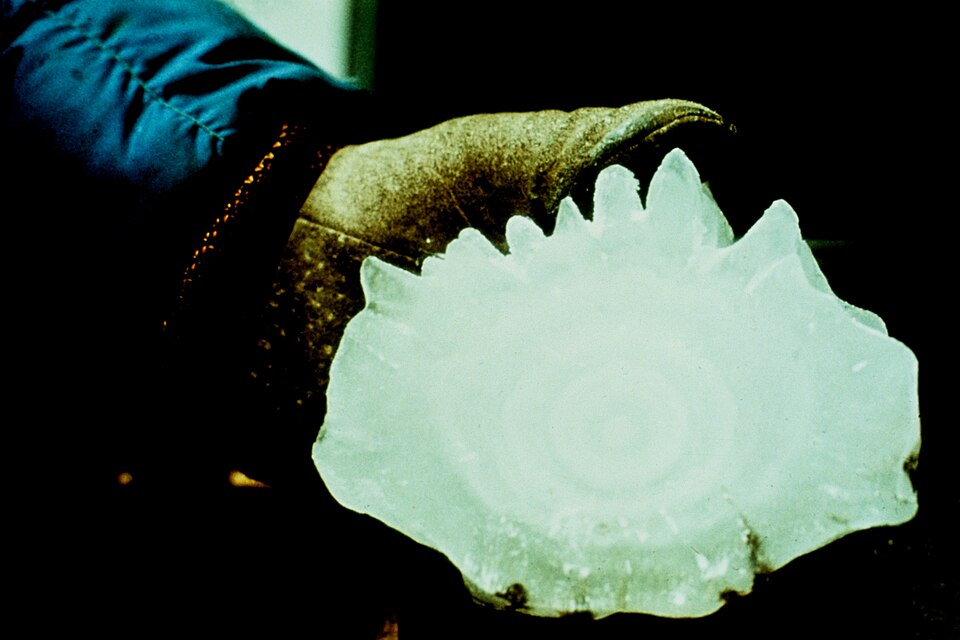
\includegraphics[width=0.5\linewidth]{images/book1/g4-hailstone.jpg}

{\small 一颗很大的\omterm{def:g4:clouds-rain-snow:precipitation}{冰雹}被戴着手套的手托着。环纹显示它
在风暴云中积聚的冰层。照片：NOAA Photo
Library（公有领域）。}
% ledger: noaa:photos-g4
\end{omfigure}

\section{测量天气}

要说明下了多少雨、\omterm{def:g1:watching-the-weather:weather}{天气}有多暖和，或风从哪个方向吹来，
只靠文字描述是不够的，还需要仪器和数字。

\begin{definition}[雨量计]\label{def:g4:clouds-rain-snow:rain-gauge}
称\emph{雨量计}\index{雨量计}为一种容器，用来收集
落在其开口上的雨水。它所收集的水的深度以
毫米为单位：“降雨 5 毫米”表示，若雨水
在平地上既未流走也未渗入，
则会形成一层深 5 毫米的水层。
\end{definition}

\begin{remark}[一毫米降雨，水量可不少]\label{rem:g4:clouds-rain-snow:litre}
一毫米降雨在\omterm{def:g4:clouds-rain-snow:rain-gauge}{雨量计}中看起来很少。但在一块边长一米的正方形地面上，
它就有一升水，相当于一大瓶。在一个校园操场上，
面积为一千平方米，降雨 10 毫米就会带来
一万升水，足以装满一千只每只 10 升的桶。
\end{remark}

\begin{omfigure}
\begin{tikzpicture}[font=\small]
  % funnel
  \draw[black!70, line width=0.8pt] (-1.2,6.6) -- (-0.35,5.8) -- (-0.35,5.4);
  \draw[black!70, line width=0.8pt] (1.2,6.6) -- (0.35,5.8) -- (0.35,5.4);
  \draw[black!70, line width=0.8pt] (-1.2,6.6) -- (1.2,6.6);
  % tube
  \fill[blue!25] (-0.45,0) rectangle (0.45,2.4);
  \draw[black!70, line width=0.8pt] (-0.45,5.4) -- (-0.45,0) -- (0.45,0) -- (0.45,5.4);
  \foreach \m in {0,1,...,50} {
    \pgfmathsetmacro{\yy}{\m*0.1}
    \draw[black!60] (0.45,\yy) -- ++(-0.12,0);
  }
  \foreach \m in {0,5,10,...,50} {
    \pgfmathsetmacro{\yy}{\m*0.1}
    \draw[black!80] (0.45,\yy) -- ++(-0.25,0);
    \node[anchor=west, font=\scriptsize] at (0.5,\yy) {\m};
  }
  \node[anchor=west, font=\scriptsize] at (1.0,5.0) {mm};
  % reading line
  \draw[red!70!black, -{Stealth}] (-1.6,2.4) -- (-0.5,2.4);
  \node[anchor=east, align=right, font=\scriptsize] at (-1.65,2.4) {在此 \\读取液面};
  \node[anchor=west, font=\scriptsize] at (1.9,2.4) {$\leftarrow$ 降雨 24\,mm};
\end{tikzpicture}

{\small 简易\omterm{def:g4:clouds-rain-snow:rain-gauge}{雨量计}：漏斗接住雨水，带刻度的细管将其盛住。读数时，
眼睛应与液面处于同一高度。图中所示为
自上次倒空\omterm{def:g4:clouds-rain-snow:rain-gauge}{雨量计}以来降下的
24 毫米雨量。}
\label{fig:g4:clouds-rain-snow:gauge}
\end{omfigure}


\begin{definition}[风向标]\label{def:g4:clouds-rain-snow:wind-vane}
称\emph{风向标}\index{风向标}为一支可在
立杆上自由转动的箭头。风吹其尾部，故箭头始终指向
风吹来的\emph{方向}。
\end{definition}

\begin{definition}[气象站]\label{def:g4:clouds-rain-snow:weather-station}
称\emph{气象站}\index{气象站}为一处每天用仪器、
以相同方式测量\omterm{def:g1:watching-the-weather:weather}{天气}的地方，仪器包括：通风白色百叶箱里的温度计、
露天的\omterm{def:g4:clouds-rain-snow:rain-gauge}{雨量计}、
立杆上的\omterm{def:g4:clouds-rain-snow:wind-vane}{风向标}。
\end{definition}

温度计放在阴凉处，所用白色箱子的四壁为百叶状，
既能让空气通过，又能挡住阳光和雨水。英国气象局
是英国的\omterm{def:g1:watching-the-weather:weather}{天气}服务机构，它将箱子设置在
离地面 \SI{1.25}{\metre} 处。\omterm{def:g4:clouds-rain-snow:rain-gauge}{雨量计}
设置在露天处，远离会挡住雨水的墙壁和树木，
其开口略高于地面。\omterm{def:g4:clouds-rain-snow:wind-vane}{风向标}则
设在高高的立杆上，高于会改变风向的障碍物。
% ledger: mo:screen-height, mo:raingauge

\begin{omfigure}
\begin{tikzpicture}[font=\small, x=1cm, y=1cm]
  % grass
  \fill[green!40!black!45] (-0.5,0) rectangle (11,-0.25);
  \foreach \x in {-0.3,0.1,...,10.8} \draw[green!45!black] (\x,0) -- ++(0.06,0.14);
  % screen on legs
  \draw[black!70, line width=1pt] (0.8,0) -- (0.8,1.25) (2.2,0) -- (2.2,1.25);
  \fill[white, draw=black!70] (0.6,1.25) rectangle (2.4,2.4);
  \foreach \y in {1.4,1.55,...,2.25} \draw[black!40] (0.7,\y) -- (2.3,\y-0.08);
  \fill[white, draw=black!70] (0.45,2.4) -- (1.5,2.75) -- (2.55,2.4) -- cycle;
  \draw[black!60, <->] (2.8,0) -- node[right, font=\scriptsize, align=left] {约 \\1.25\,m} (2.8,1.25);
  \node[align=center, font=\scriptsize] at (1.5,3.25) {白色百叶箱中的 \\温度计};
  % rain gauge
  \fill[black!15, draw=black!70] (5.4,0) rectangle (5.9,0.4);
  \draw[black!70] (5.3,0.55) -- (5.4,0.4) (6.0,0.55) -- (5.9,0.4);
  \node[align=center, font=\scriptsize] at (5.65,1.2) {露天的 \\雨量计};
  % tree far away
  \fill[brown!60!black] (7.3,0) rectangle (7.5,1.3);
  \fill[green!50!black!70] (7.4,2.1) circle (0.85);
  % wind vane on a mast
  \draw[black!70, line width=1pt] (9.8,0) -- (9.8,4.2);
  \draw[black!80, line width=1.4pt, -{Latex[length=3mm]}] (10.6,4.4) -- (9.0,4.4);
  \fill[black!80] (10.6,4.4) -- (10.9,4.65) -- (10.9,4.15) -- cycle;
  \node[align=center, font=\scriptsize] at (9.8,5.05) {高立杆上的风向标};
  \node[anchor=west, font=\scriptsize, align=left] at (10.1,3.4) {指向 \\风吹来的方向};
\end{tikzpicture}

{\small 小型\omterm{def:g4:clouds-rain-snow:weather-station}{气象站}。温度计位于阴凉处的白色
百叶箱中，箱子四壁为百叶状，距草地约 1.25 米；\omterm{def:g4:clouds-rain-snow:rain-gauge}{雨量计}
设在露天处，远离树木；\omterm{def:g4:clouds-rain-snow:wind-vane}{风向标}高高地位于
障碍物之上。}
\label{fig:g4:clouds-rain-snow:station}
% ledger: mo:screen-height
\end{omfigure}

\begin{inthefield}[学校操场上的气象站]
许多学校会在操场的一角设立一个小型\omterm{def:g4:clouds-rain-snow:weather-station}{气象站}。
每天早上同一时间，两名学生看温度计，
读取并清空\omterm{def:g4:clouds-rain-snow:rain-gauge}{雨量计}，记下\omterm{def:g4:clouds-rain-snow:wind-vane}{风向标}指向的方向。几周下来，
全班便积累起属于自己的\omterm{def:g1:watching-the-weather:weather}{天气}记录。
\end{inthefield}

\begin{omfigure}
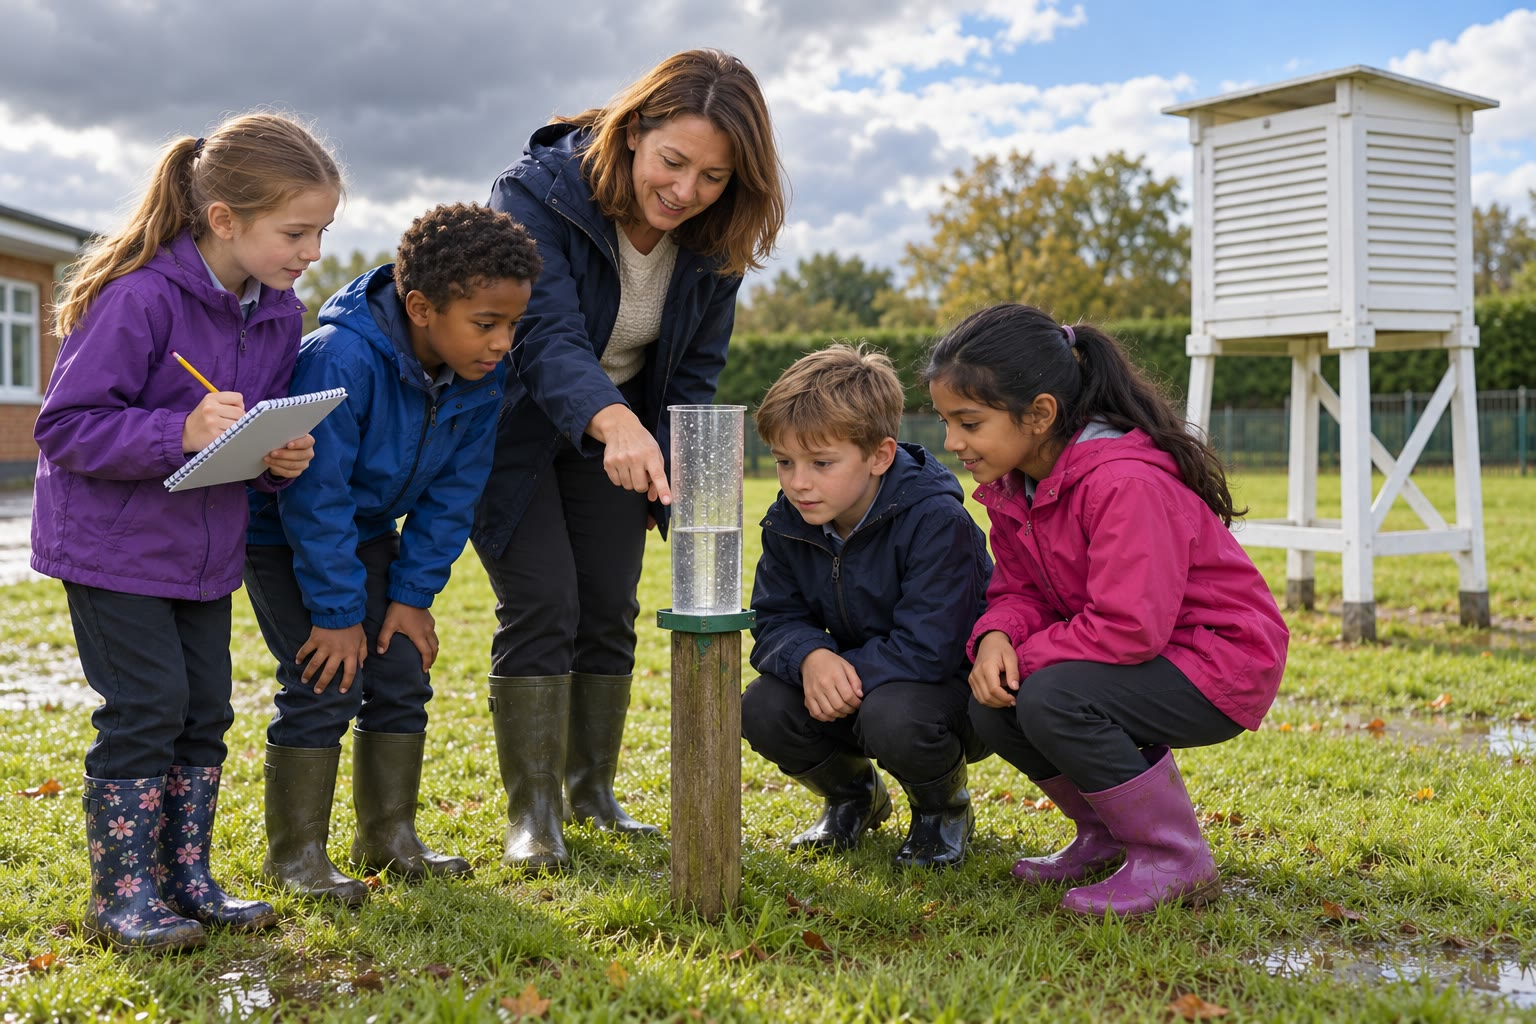
\includegraphics[width=0.55\linewidth]{images/book1/ai/g4-rain-gauge-class.jpg}

{\small 学生在学校操场上读取\omterm{def:g4:clouds-rain-snow:rain-gauge}{雨量计}。}
\end{omfigure}

\begin{method}[画出降雨量的柱状图]\label{met:g4:clouds-rain-snow:bar-chart}
要画出一周的降雨量：
\begin{enumerate}
  \item 画一条水平线，在线下按相等间距写上各天的名称；
  \item 在左侧画一条竖线，并以毫米为单位标出刻度，
        刻度间隔相等（例如每 2 毫米一格）；
  \item 在每一天的上方画一根柱子，柱子高度与当天降雨量相同；
        无雨的那天不画柱子；
  \item 为图表加上标题，并在竖线上
        标明单位 mm。
\end{enumerate}
\end{method}

\begin{example}[学校一周的降雨量]\label{ex:g4:clouds-rain-snow:week}
全班每天早上读取\omterm{def:g4:clouds-rain-snow:rain-gauge}{雨量计}，一周的记录为：周一 0，
周二 4，周三 12，周四 7，周五 0，周六 2，周日 5 毫米。
降雨最多的是周三。周一和周五都没有下雨。
一周内共降雨 $0 + 4 + 12 + 7 + 0 + 2 + 5 = 30$ 毫米。
周三一天就降了其中的 12 毫米，即
$\frac{12}{30} = \frac{2}{5}$，占全周降雨量的五分之二。
\end{example}

\begin{omfigure}
\begin{tikzpicture}
\begin{axis}[ybar, bar width=14pt, width=0.8\linewidth, height=5.4cm,
    ymin=0, ymax=14, ytick={0,2,...,14}, ylabel={降雨量 (mm)},
    symbolic x coords={Mon,Tue,Wed,Thu,Fri,Sat,Sun}, xtick=data, xticklabels={周一,周二,周三,周四,周五,周六,周日},
    axis x line*=bottom, axis y line*=left, ymajorgrids, grid style={gray!25},
    nodes near coords, nodes near coords style={font=\scriptsize},
    every axis label/.append style={font=\small}, tick label style={font=\small},
    title={学校一周的降雨量}, title style={font=\small}]
  \addplot[fill=omWxRain!70, draw=omWxRain!60!black] coordinates
    {(Mon,0) (Tue,4) (Wed,12) (Thu,7) (Fri,0) (Sat,2) (Sun,5)};
\end{axis}
\end{tikzpicture}

{\small \cref{ex:g4:clouds-rain-snow:week} 的柱状图。}
\label{fig:g4:clouds-rain-snow:bars}
\end{omfigure}

\section{练习}

\begin{exercise}[$\star$]\label{exo:g4:clouds-rain-snow:1}
云是由什么组成的？雾是什么？
\end{exercise}

\begin{exercise}[$\star$]\label{exo:g4:clouds-rain-snow:2}
说出下列云的名称：(a) 覆盖整个天空的扁平灰色\omterm{def:g4:clouds-rain-snow:cloud}{云层}；(b) 蓝天高处的
细白丝缕；(c) 底部平坦、如棉花团般的白色云堆；
(d) 带来雷声的巨大深色云塔，顶部平坦。
\end{exercise}

\begin{exercise}[$\star$]\label{exo:g4:clouds-rain-snow:3}
雨、雪还是\omterm{def:g4:clouds-rain-snow:precipitation}{冰雹}？(a) 从风暴云中落下的冰球；(b) 液态的
水滴；(c) 由冰晶组成的雪花。
\end{exercise}

\begin{exercise}[$\star$]\label{exo:g4:clouds-rain-snow:4}
下列仪器分别用来测量什么？(a) 降雨量；(b) 温度；
(c) 风从哪个方向来。
\end{exercise}

\begin{exercise}[$\star$]\label{exo:g4:clouds-rain-snow:5}
在第~\pageref{fig:g4:clouds-rain-snow:gauge}~页所示的\omterm{def:g4:clouds-rain-snow:rain-gauge}{雨量计}中，水位现在
到达刻度 17。已降了多少毫米的雨？
还需再降多少毫米，水位才能达到 20？
\end{exercise}

\begin{exercise}[$\star$]\label{exo:g4:clouds-rain-snow:6}
看一看第~\pageref{fig:g4:clouds-rain-snow:bars}~页的柱状图。哪一天
降雨最多？哪几天没有下雨？哪一天降了 7
毫米？
\end{exercise}

\begin{exercise}[$\star\star$]\label{exo:g4:clouds-rain-snow:7}
在一个下雪的早晨，雪花在山村
落到地面，而山下的\omterm{def:g1:landscapes-around-us:landform}{山谷}却在下雨。请解释其中的差异，
并结合空气的温度加以说明。
\end{exercise}

\begin{exercise}[$\star\star$]\label{exo:g4:clouds-rain-snow:8}
另一周，全班记录的数据为：周一 3，周二 0，周三 1，周四
9，周五 6，周六 0，周日 1 毫米。请画出柱状图。这一周共
降雨多少毫米？全周降雨量中，落在周四的
那部分占几分之几？
\end{exercise}

\begin{exercise}[$\star\star$]\label{exo:g4:clouds-rain-snow:9}
为什么\omterm{def:g4:clouds-rain-snow:rain-gauge}{雨量计}必须放在空旷处，远离墙壁和树木？为什么
温度计要放在阴凉处的白色箱子里，而不放在阳光直射处？
\end{exercise}

\begin{exercise}[$\star\star$]\label{exo:g4:clouds-rain-snow:10}
\omterm{def:g4:clouds-rain-snow:wind-vane}{风向标}指向西方。风从哪里来？风
要往哪里去？
\end{exercise}

\begin{exercise}[$\star\star\star$]\label{exo:g4:clouds-rain-snow:11}
在面积为 500 平方米的操场上，降雨 8 毫米。利用
\cref{rem:g4:clouds-rain-snow:litre}，计算操场上降落了多少升水？一个
洒水壶能装 10 升水，这相当于多少个洒水壶？
\end{exercise}
